\newcommand{\dsename}[1]{\textit{#1}}

\vspace{-2pt}
\subsection{MAAR DSE Flow and Traversal}
\label{subsec:MAAR}

Novel exploration approaches are needed that broaden the scope of DSE from single application to a set of applications in order to design a MAAR platform. The enormous design space renders exhaustive search unfeasible, requiring heuristics for sparse sampling. MAAR DSE employs an elitist Genetic Algorith (GA)~\cite{quan2014towards} to support efficient design space traversal.

%\vspace{-4pt}
\begin{figure}[h]
	\centering
	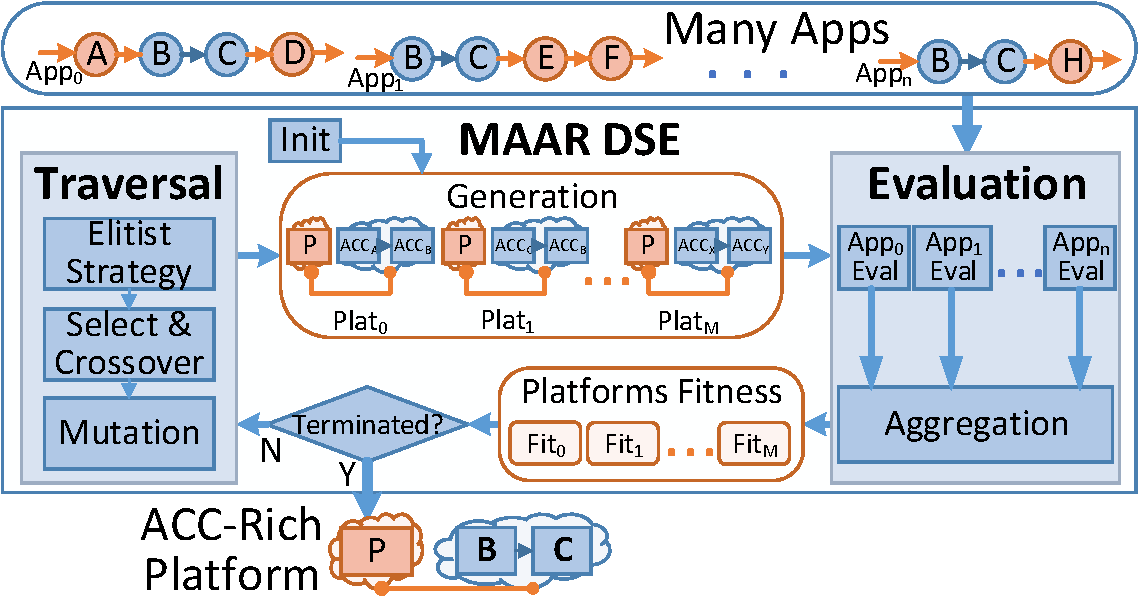
\includegraphics[width=.9\linewidth]{fig/MAARflowDetial.pdf}
	\vspace{-4pt}
	\caption{MAAR Detial Flow}
	\label{fig:MAARflowDetial}
\end{figure}

\figref{fig:MAARflowDetial} overviews MAAR DSE flow. The exploration configuration (one generation) is captured in a set of chromosomes, representing platforms. Each chromosome captures platform allocation of kernels across many applications as a set of genes. After randomly generating an initial generation, the MAAR \dsename{Evaluation} analyzes the fitness of each chromosome/platform. In \dsename{Traverse}, the \dsename{Elitist Strategy} tracks global top 10\% platforms (across all generations). It replaces the bottom 10\% each generation with the global top 10\%. From this, \dsename{Selection \& Crossover} selects pairs of promising chromosomes with roulette wheel selection according to their fitness and swaps genes among them. To further speed up exploration, \dsename{Mutation} employs a local search method guided by analytic evaluation to propagate the best neighbor of the design point. The resulting generation is evaluated and the process repeats until the \dsename{Termination} condition (no better platform for 10 iterations) is reached.